\documentclass[10pt]{article}
\usepackage[preprint]{tmlr}
\usepackage{amsmath,amssymb,graphicx,booktabs}
\usepackage[hidelinks]{hyperref}
\usepackage{url}
\urlstyle{same}
\providecommand{\doi}[1]{\href{https://doi.org/#1}{doi:~\nolinkurl{#1}}}
\DeclareMathOperator{\sgn}{sign}
\title{Supervised Hebbian Class Networks: Regression Without Backpropagation}
\author{}
\begin{document}
\maketitle

\begin{abstract}
We extend the classifier introduced in \emph{Supervised Hebbian Class Networks: Learning Without Backpropagation} to regression. The sign of the final prediction error supplies a teaching signal to every layer. Each connection learns from that sign and the activities of the neurons it connects. Neurons can reinforce or suppress their activity on different examples. For a large output vector, each hidden neuron combines the error signs from a group of outputs. We demonstrate the approach on scalar curve fitting, implicit representation of an image, and image generation using an autoencoder.
\end{abstract}

\section{Regression from Class Network}
We extend the supervised Hebbian classifier of \citet{loverich2026} to regression. The classifier uses the target label and the strongest competing label to decide which classes to reinforce and suppress. For regression we treat each quantity to be predicted as an \emph{output class}. Each class has a numerical target. The class error tells the network whether to increase or decrease its prediction. The curve has one class. Blue Marble has three classes, one per color at the supplied coordinates. The CelebA autoencoder has $64\times64\times3=12{,}288$ classes, one per color channel at each image position. It predicts a value for every class in one forward pass.

In the curve and implicit image models, each neuron contributes its signed activity $h$ to one class. Its contribution can be positive on one input and negative on another. When the prediction is too low, the learning rule reinforces positive activities and suppresses negative activities. When the prediction is too high, the directions reverse. Figure~\ref{fig:network} illustrates this rule for a scalar output. The Blue Marble network applies the same rule separately to red, green and blue. In the CelebA autoencoder, each hidden neuron receives a weighted sum of error signs from a fixed subset of the 12,288 classes. Each output neuron predicts one class and receives its error sign.

\begin{figure}[!ht]
\centering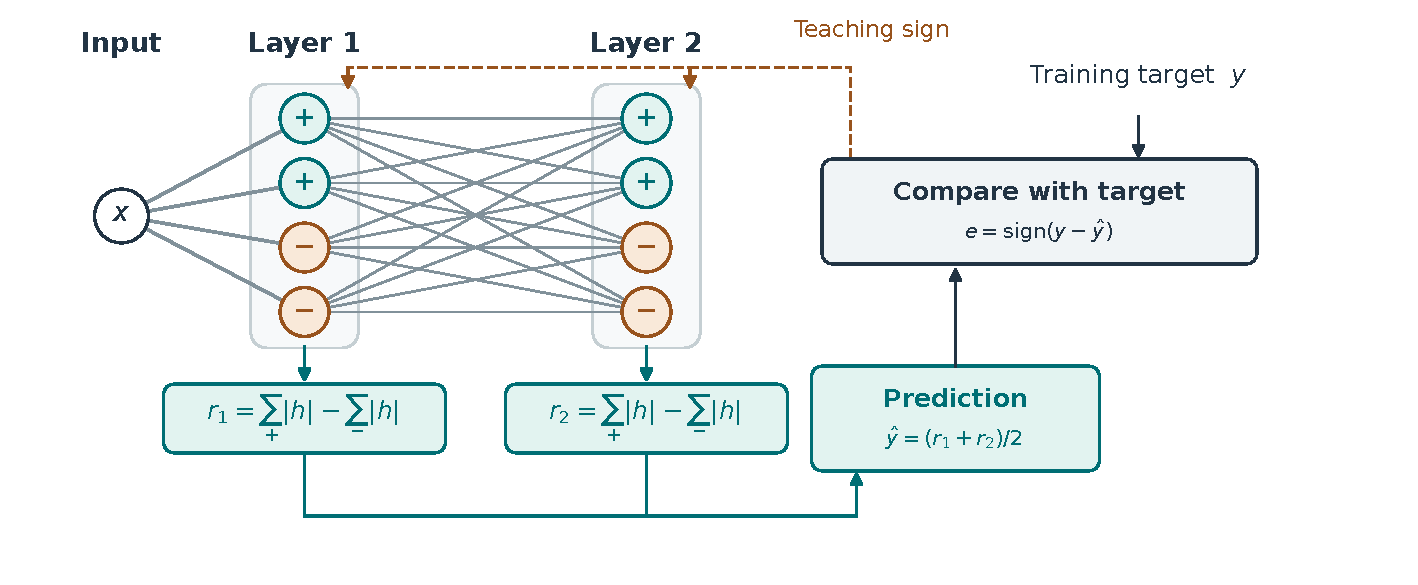
\includegraphics[width=.92\linewidth]{figures/class-network.pdf}
\caption{A scalar regressor with two fully connected layers. Each layer sums its signed neuron activities to give an estimate $r_1$ or $r_2$. The prediction is their average. Dashed arrows send the sign $e$ of the final prediction error to all layers during training.}
\label{fig:network}
\end{figure}

\section{Forward pass with competitive activations and signed pooling}
\label{sec:prediction}
For a vector of $K$ continuous targets, the network estimates all $K$ values in one forward pass.

Let $u$ be the input to one dense layer. The first layer receives the supplied input vector, and each subsequent layer receives the activities from its predecessor. Neuron $j$ computes $z_j=b_j+\sum_i w_{ij}u_i$. The layer then compares magnitudes within a group of neurons, called a \emph{competition pool}. The input weights remain dense across pool and class boundaries. With hard top-$k$ selection, the $k$ neurons with the largest $|z_j|$ in each pool retain their signed activities. The remaining activities are set to zero.

For Gaussian competition, the reference magnitude $m$ is the largest $|z_j|$ in the pool for this example. A Gaussian of width $\tau>0$ scales the signed activity of every neuron in the pool,
\begin{equation}
 h_j=z_j\exp(-d_j^2/2), \qquad
 d_j=\min\!\left(13,\frac{\big|m-|z_j|\big|}{m\tau}\right).
 \label{eq:competition}
\end{equation}
An all-zero pool returns zeros. A neuron at the reference magnitude retains its full activity. A neuron one width away retains about 61\%. The cap keeps the Gaussian factor representable in the arithmetic used here.

In the coordinate regressors, let $P_{\ell k}$ be the neurons that estimate output $k$ in layer $\ell$. Each layer gives one estimate and the network averages them over all $L$ layers,
\begin{equation}
 r_{\ell k}=\sum_{j\in P_{\ell k}} h_j,
 \qquad
 a_k=\frac{1}{L}\sum_{\ell=1}^{L} r_{\ell k}.
 \label{eq:output}
\end{equation}
For scalar regression the prediction is $\hat y_k=a_k$. For the implicit image representation, we clip $a_k$ to $[-1,1]$ and round to the nearest of 256 equally spaced values in that interval. We apply the same conversion to the target.

The CelebA decoder predicts each channel from one dense output neuron. Its signed activity is $h_k=b_k+\sum_i w_{ik}u_i$, where $u$ contains the activities of the final hidden layer. On the RGB intensity scale $[0,1]$, its prediction is
\begin{equation}
 \hat I_k=\frac{\operatorname{round}\!\left(255\min(1,|h_k|)\right)}{255}.
 \label{eq:intensity}
\end{equation}
For training we express this intensity on the same scale as the input image, $\hat y_k=2\hat I_k-1$. The output neuron receives the teaching signal $s_k=e_k$, where $e_k$ is the sign of the target minus the prediction (Eq.~\ref{eq:sign}). Because the local update uses the signed $h_k$, a positive teaching sign reinforces activity of either sign and a negative teaching sign suppresses it.

We initialize weights and biases independently from zero-mean normal distributions with standard deviations $1/\sqrt{F}$ and $0.35$, respectively, where $F$ counts the inputs to the neuron. For the CelebA autoencoder, we multiply the initial weights and biases of the RGB output layer by $0.12$.

\section{Supervised Hebbian learning from output error signs}
For each example the network computes the complete prediction, then compares it with the target in each output coordinate,
\begin{equation}
 e_k=\sgn(y_k-\hat y_k),\qquad \sgn(0)=0 .
 \label{eq:sign}
\end{equation}
For a neuron $j$ that contributes its signed activity to output $k$, set $s_j=e_k\sgn(h_j)$. When $e_k=+1$, the neuron receives $s_j=+1$ if its contribution is positive and $s_j=-1$ if its contribution is negative. Its signed coactivity then uses $h_js_j=|h_j|e_k$. A neuron that predicts an intensity through its magnitude receives $s_j=e_k$. In both rules the final prediction supplies the error sign.

\paragraph{Joint training.} Each minibatch passes through all layers before any weight changes. Every layer computes its update from the activities recorded on that pass and the signs of the errors in the final prediction. In the autoencoder this includes the encoder, the bottleneck layer and the decoder from the first minibatch onward.
\begin{enumerate}
\item Pass every example through the network. Save the input and activity of each neuron.
\item Pool the activities into output values. Compare each final output with its target to obtain $e_k$.
\item Compute the teaching signal $s_j$ for each neuron. For autoencoder hidden neurons, combine the output signs as in Section~\ref{sec:grouped-signs}.
\item At each neuron, average the signed activity products and squared activities over contributing examples. Update its incoming weights and bias using the chosen Lion rule. The next minibatch uses the updated network.
\end{enumerate}

\subsection{Minibatch estimates of signed coactivity and squared activity}
For a connection from input $i$ to neuron $j$, each contributing example supplies the signed activity product $u_i h_j s_j$. With $u_i>0$, $h_j<0$, and $s_j=+1$, this example contributes a negative term to the minibatch average $A_{ij}$.

Let $B_j$ be the examples in a minibatch for which $s_j$ and $h_j$ are both nonzero. Using $b$ to index an example, calculate
\begin{equation}
 A_{ij}=\frac{1}{|B_j|}\sum_{b\in B_j}u_{bi}h_{bj}s_{bj},
 \qquad
 Q_j=\frac{1}{|B_j|}\sum_{b\in B_j} h_{bj}^2 .
 \label{eq:observations}
\end{equation}
Here $A_{ij}$ measures signed coactivity and $Q_j$ measures how strongly the receiving neuron was active. Skip the neuron when $B_j$ is empty. Treat the bias as one more weight with a constant input of one.

\subsection{Hebbian Lion weight updates}
The Hebbian adaptation of Lion \citep{loverich2026,chen2023} combines the current coactivity $A_{ij}$ with its running average $M_{ij}$ to choose an update direction. For an active neuron, compute $S_{ij}$ using the old $M_{ij}$, then update the running average,
\begin{equation}
 S_{ij}=0.125 M_{ij}+0.875 A_{ij},\qquad
 M_{ij}\leftarrow 0.99 M_{ij}+0.01 A_{ij}.
 \label{eq:history}
\end{equation}
The running average starts at zero. An inactive neuron retains its previous average and weights.

Let $d_{\rm in}$ count the inputs to a neuron, including the constant input for its bias. Following Equation~(7) of \citet{loverich2026}, set $D_{ij}=\sgn(S_{ij})/\sqrt{d_{\rm in}}$. For a step size $\eta$, the semi-implicit update is
\begin{equation}
 w_{ij}\ \leftarrow\
 \frac{w_{ij}+\eta D_{ij}}{1+\eta Q_j}.
 \label{eq:update}
\end{equation}
The division by $\sqrt{d_{\rm in}}$ bounds the length of the signed step across all incoming weights of a neuron by $\eta$. The denominator shrinks the incoming weights more strongly at a neuron with larger squared activity. The explicit form is $w_{ij}\leftarrow w_{ij}+\eta D_{ij}-\eta Q_j w_{ij}$, with the weight before the minibatch in the last term. Both forms follow \citet{loverich2026}. \citet{oja1982} used the receiving neuron's squared activity to control weight growth.

Each run uses the same update throughout training. The target supplies only the sign in Equation~\ref{eq:sign}. Given its teaching signal, each neuron updates its incoming weights from the activities at the two ends of each connection. The output comparison itself requires information from the whole network.

\subsection{Per-neuron step sizes from sign agreement}
In preliminary fits of the Blue Marble image with a 12-layer MLP, assigning smaller steps to layers closer to the input reduced the summed squared pixel error compared with using the same step in every layer. This motivated a rule that adjusts the step size of each neuron during training, so the effective steps can vary across layers without specifying a rate for each layer.

In the adaptive form of semi-implicit Lion, all layers share the cosine step-size schedule $\eta_t$. Each receiving neuron $j$ keeps a step multiplier $g_j$, initialized to one. For each active neuron, $a_{j,t}$ is the average sign agreement between the current coactivity $A_{ij}$ and the old history $M_{ij}$ over its $d_{\rm in}$ incoming weights, including the bias. Matching nonzero signs count as $+1$, opposite signs as $-1$, and a zero on either side counts as $0$. This average is over weights within minibatch $t$. The multiplier $g_{j,t}$ carries over from one minibatch to the next.
\begin{equation}
 a_{j,t}=\frac{1}{d_{\rm in}}\sum_i\sgn(M_{ij})\sgn(A_{ij}),
 \qquad g_{j,t}=\operatorname{clip}\!\left(g_{j,t-1}\,0.99^{-a_{j,t}},\,0.01,\,1\right).
 \label{eq:agreement}
\end{equation}
For example, if 40\% of the incoming weights agree and 60\% disagree, then $a_{j,t}=-0.2$. One such minibatch multiplies the previous step multiplier by $0.99^{0.2}\approx0.998$. Starting from one, 2,292 such updates reach the lower bound of $0.01$. Positive agreement on intervening minibatches offsets some of this decrease, up to the upper bound of one. On minibatch $t$, every incoming weight of neuron $j$, including its bias, takes the same step size $\eta_t g_{j,t}$. The adaptive semi-implicit weight update is
\begin{equation}
 w_{ij,t}=\frac{w_{ij,t-1}+\eta_t g_{j,t} D_{ij}}{1+\eta_t g_{j,t} Q_j}.
 \label{eq:adaptive-update}
\end{equation}
Here $D_{ij}$ and $Q_j$ are the direction and mean squared activity for the current minibatch. A neuron with no contributing examples keeps its previous multiplier and weights.

\subsection{Grouping output errors to teach a narrower layer}
\label{sec:grouped-signs}
In the CelebA autoencoder, each hidden neuron $j$ has a signed activity $h_j$ and a fixed set $G_j$ of output classes. Each class in $G_j$ contributes its error sign to the teaching signal for that neuron. The number of assigned classes $N=|G_j|$ depends on the layer. For example, each of the 256 bottleneck neurons receives signs from 96 of the 12,288 classes (Fig.~\ref{fig:auto}).

In each hidden layer, we shuffle the output indices and divide them among half as many groups as neurons. We use the largest even group size that fits and set aside any remainder. We independently shuffle and partition the same covered indices a second time, then shuffle the groups from both partitions and assign one group to each neuron. These assignments remain fixed throughout training. Each layer is fully connected to the preceding layer regardless of the group assignments. Every covered output therefore teaches two neurons in the layer. Half of the indices $k$ in each group have a fixed multiplier $v_{jk}=+1$ and half have $v_{jk}=-1$. The grouping uses only the output indices.

\begin{figure}[!ht]
\centering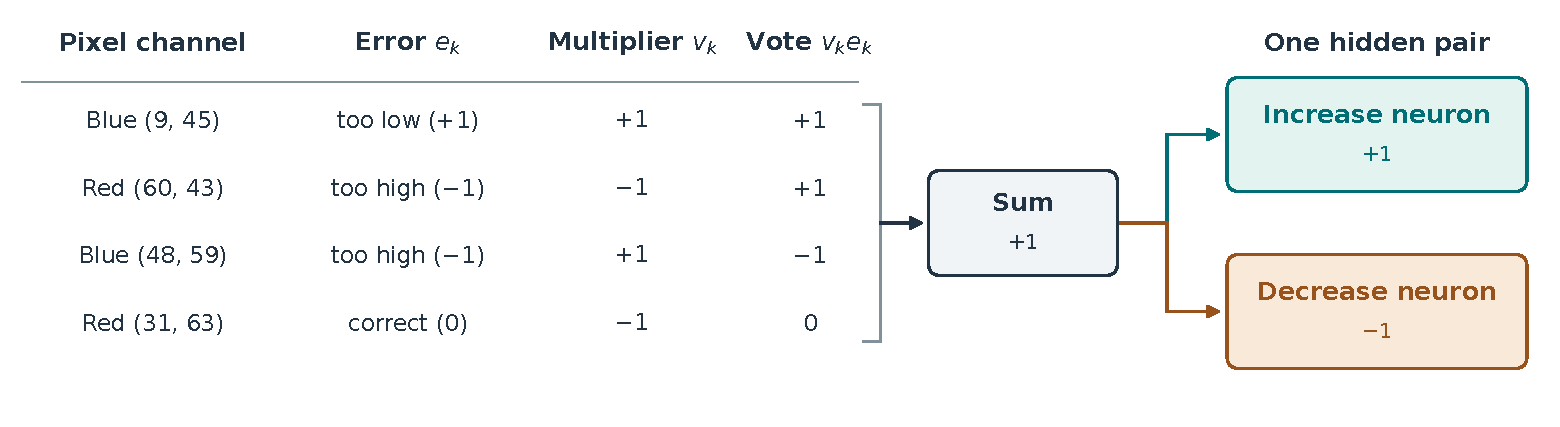
\includegraphics[width=.96\linewidth]{figures/pixel-votes.pdf}
\caption{Four of the 96 channels assigned to one bottleneck neuron. Suppose the other 92 match their targets. The three nonzero votes sum to $+1$, which multiplies the neuron's local activity product on this example.}
\label{fig:pixel-votes}
\end{figure}

For image $b$, the teaching signal is the vote sum $t_{bj}=\sum_{k\in G_j}v_{jk}e_{bk}$. Let $c_{bj}=\sum_{k\in G_j}|e_{bk}|$ count the incorrect intensities in that group. Opposite votes cancel in $t_{bj}$ and both count in $c_{bj}$. The total number of votes received while neuron $j$ was active is $C_j=\sum_{b:\,h_{bj}\ne0}c_{bj}$. We use this total to average the minibatch observations,
\begin{equation}
 A_{ij}=\frac{1}{C_j}\sum_b u_{bi}h_{bj}t_{bj},\qquad
 Q_j=\frac{1}{C_j}\sum_b c_{bj} h_{bj}^2 .
 \label{eq:votes}
\end{equation}
Skip the update if $C_j=0$. The output neurons use Equation~\ref{eq:observations} directly, with $s_k=e_k$.

\section{Experimental Results}
Table~\ref{tab:output-classes} gives the class count for each experiment. In the CelebA network, 256 bottleneck neurons receive teaching signals from all 12,288 classes collectively. Each individual bottleneck neuron uses only 96 of them.

\begin{table}[!ht]
\centering
\caption{Output classes in the three regression problems. The last column gives the number of classes whose error signs teach one hidden neuron.}
\label{tab:output-classes}
\begin{tabular}{@{}l r l l@{}}
\toprule
Experiment & Classes & One class predicts & Classes per hidden neuron\\
\midrule
Sine fit & 1 & Curve value at $x$ & 1\\
Blue Marble & 3 & One color at $(x,y)$ & 1 (its assigned color)\\
CelebA autoencoder & 12,288 & One color at one image position & 8, 16, 96, 12 in layer order\\
\bottomrule
\end{tabular}
\end{table}

\subsection{1D Curve Fitting}
We test how well the Hebbian rule trains a plain, fully connected multilayer perceptron (MLP) to follow a curve with a jump. One set of weights serves the whole interval. A sinusoidal representation network (SIREN) can express a sine wave with one sine unit and an output scale \citep{sitzmann2020}. \citet{lane1990} used B-splines for the connections in an MLP.

For $x\in[-1,1]$ the target is $0.5\sin(2\pi x)$ through $x=0.25$ and $0.5\sin(2\pi x)+0.5$ thereafter. Its value jumps from $0.5$ to $1$ where both branches have zero limiting slope. The network receives only $x$. We assign 12,288 equally spaced cell centers cyclically to training, validation and test sets of 4,096 points each. The validation points select checkpoints. Test points measure interpolation.

Each layer has one competition pool. We train signed-activity networks at four sizes (Table~\ref{tab:sine}). The multilayer models use Gaussian widths from $0.32$ to $0.16$ across layers, and the single-layer model uses $0.32$. We train for 640 epochs in batches of 64 with adaptive semi-implicit Lion. The shared step starts at $0.00075$ and decays along one half cosine. We evaluate checkpoints every five epochs and retain the one with the lowest validation error. The single-layer fit misses the jump. Among the width-64 networks, median test error decreases from 0.03095 at four layers to 0.01141 at 24 layers.

\begin{figure}[ht]
\centering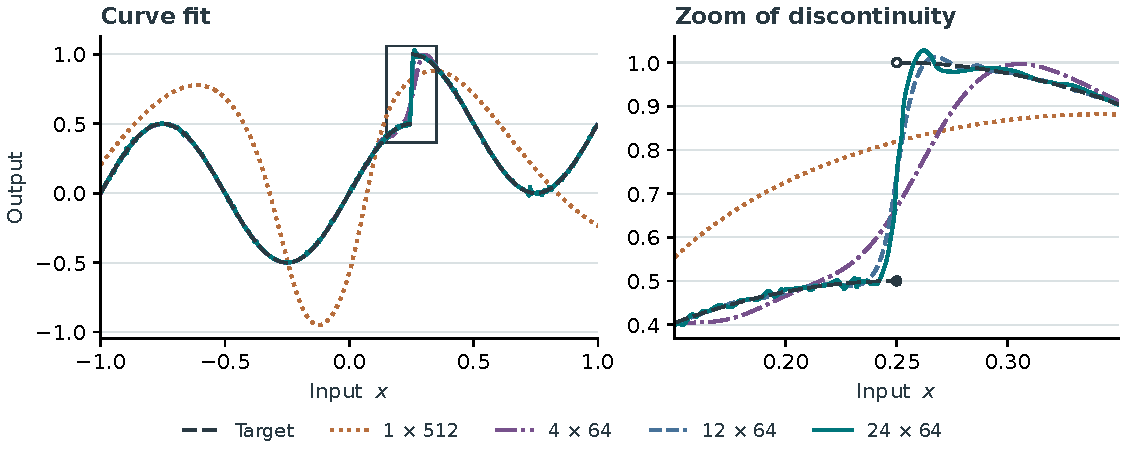
\includegraphics[width=\linewidth]{figures/sine.pdf}
\caption{Discontinuous sine and the four signed-activity networks. Each curve shows the run with the median test error for that size. The legend gives hidden layer count $\times$ width. The right panel magnifies the region marked at left.}
\label{fig:sine}
\end{figure}

\begin{table}[ht]
\centering
\caption{Discontinuous sine. Test root mean squared error (RMSE) is the median over three fits.}
\label{tab:sine}
\begin{tabular}{@{}lrr@{}}
\toprule
Hidden layers $\times$ width & Parameters & Test RMSE\\
\midrule
$1\times512$ & 1,024 & 0.26120\\
$4\times64$ & 12,608 & 0.03095\\
$12\times64$ & 45,888 & 0.01592\\
$24\times64$ & 95,808 & 0.01141\\
\bottomrule
\end{tabular}
\end{table}

\newpage
\subsection{Implicit Representation of an Image}
We train a plain MLP to represent a photograph as a function from image coordinates to RGB values. One set of weights serves the whole image. For applications that need a compact image representation, SIRENs offer a specialized alternative. \citet{sitzmann2020} used sine activations to recover fine image detail from pixel coordinates.

The input is a position $(x,y)$ on a $128\times128$ grid spanning $[-1,1]^2$. Each target is the RGB triple at that point in a crop of the Apollo 17 Blue Marble photograph \citep{nasa1972}. Each of the 12 layers has three Gaussian competition pools of 144 neurons, one per color. Gaussian widths range from $0.24$ to $0.08$ across layers. There are 2,058,912 learned weights and biases.

For each position the network computes three error signs $(e_R,e_G,e_B)$. A neuron $j$ in the red pool receives only the red error sign and uses $s_j=e_R\sgn(h_j)$ in its update. The green and blue pools use $e_G$ and $e_B$ in the same way (Fig.~\ref{fig:implicit-image}). A neuron in any of the three pools receives inputs from all three pools in the preceding hidden layer. We train and evaluate on all 16,384 pixels. Training uses adaptive semi-implicit Lion for 560 epochs in batches of 128. The shared step starts at $0.004$ and decays along one half cosine. Every neuron uses the same rule in Equation~\ref{eq:agreement}. We retain the checkpoint with the lowest error on the complete image, evaluating every five epochs. The final checkpoint gives the lowest error.

\begin{figure}[!ht]
\centering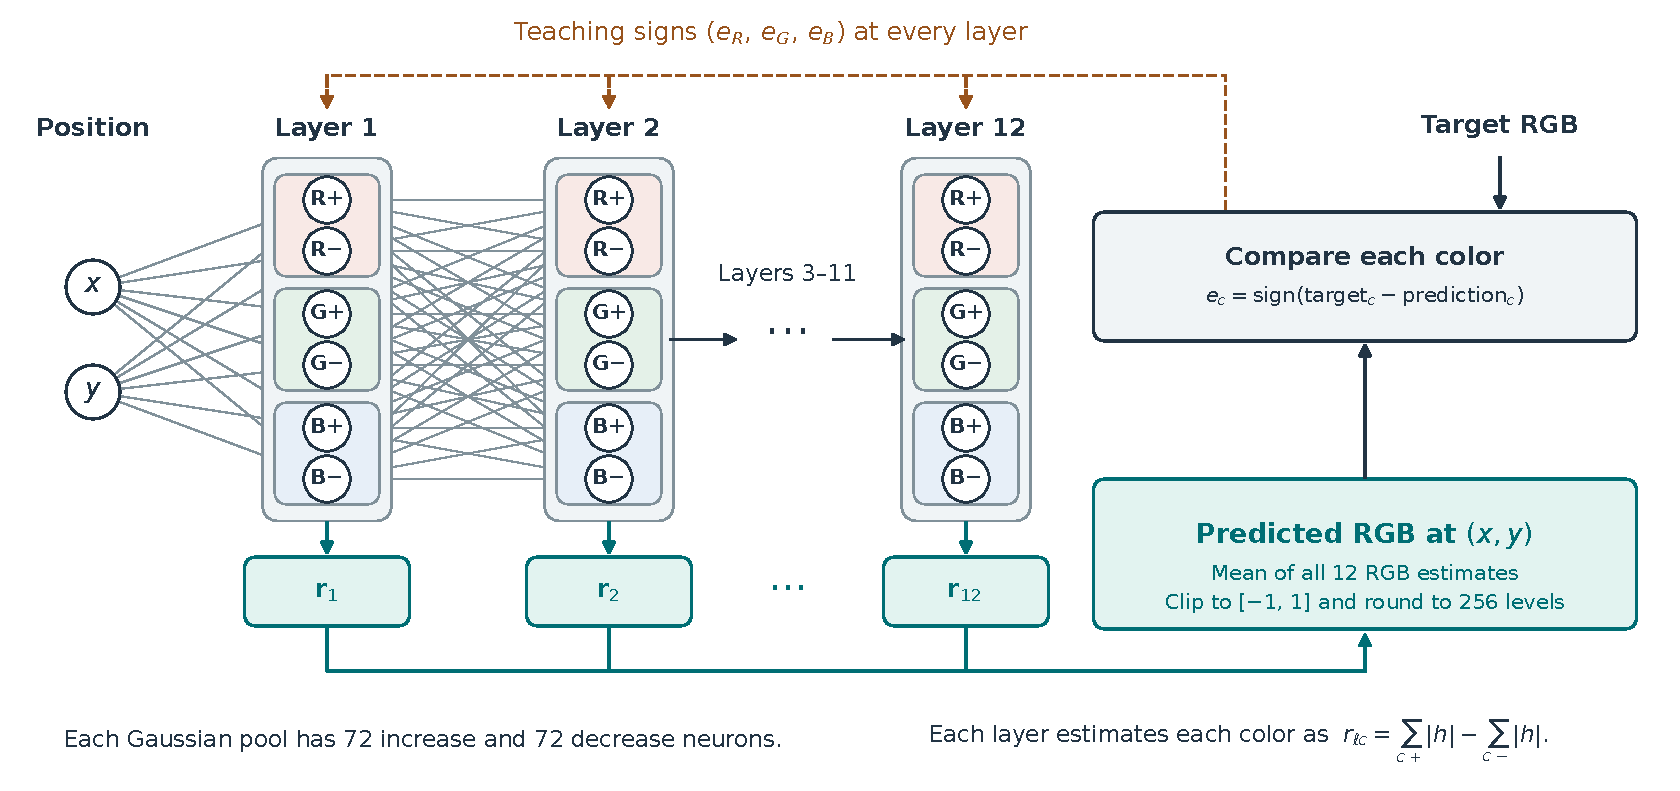
\includegraphics[width=\linewidth]{figures/implicit-image.pdf}
\caption{Blue Marble network for one pixel position. Each layer is fully connected to the preceding layer and sums its signed neuron activities separately for each color. The dashed path carries the final error signs to the corresponding pools during training.}
\label{fig:implicit-image}
\end{figure}

\begin{figure}[ht]
\centering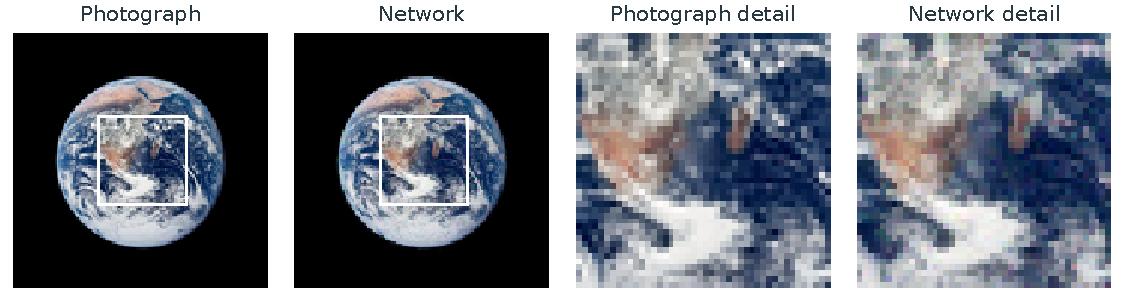
\includegraphics[width=\linewidth]{figures/earth.pdf}
\caption{The Blue Marble photograph and the RGB values predicted from its coordinates. The two right panels enlarge the same $44\times44$ region marked at left. Photograph courtesy of NASA Johnson Space Center.}
\label{fig:earth}
\end{figure}

With RGB values expressed on $[0,1]$, the sum of squared differences across all 49,152 channel values is 9.22.

\newpage
Figure~\ref{fig:earth-layers} shows how each layer contributes to the reconstruction.

\begin{figure}[!htb]
\centering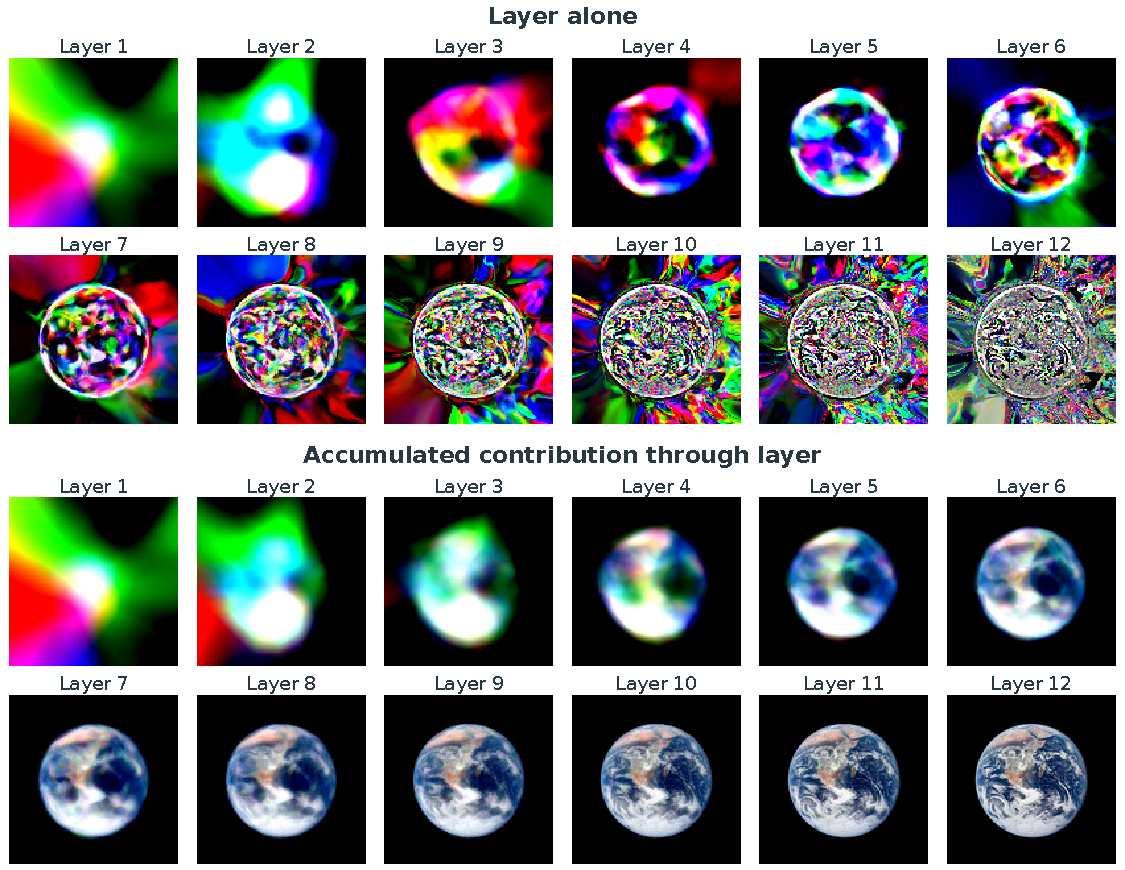
\includegraphics[width=\linewidth]{figures/earth-layers.pdf}
\caption{Blue Marble from the trained network. The top two rows show each layer's own RGB estimate $r_{\ell}$, in order from 1 to 12. The bottom two rows show the accumulated contribution through each layer in the same order, $(r_1+\cdots+r_{\ell})/\ell$. Each image uses the activities from the same forward pass at each pixel. We clip and round after computing the displayed estimate. The lower right image is the full reconstruction in Figure~\ref{fig:earth}.}
\label{fig:earth-layers}
\end{figure}

\newpage
\subsection{Image Generation Using a Dense Autoencoder}
The encoder maps an image to a 256-value embedding, and the decoder reconstructs the image from that embedding. Here the reconstruction supplies all the teaching signs. We use the official CelebA training split of 162,770 aligned photographs \citep{liu2015}. We crop each image to a centered square, resize it to $64\times64$ with Lanczos resampling, and scale the RGB values to $[-1,1]$. The encoder subtracts the training-set mean at each of the 12,288 input positions. The target is the scaled, uncentered image.

\begin{figure}[ht]
\centering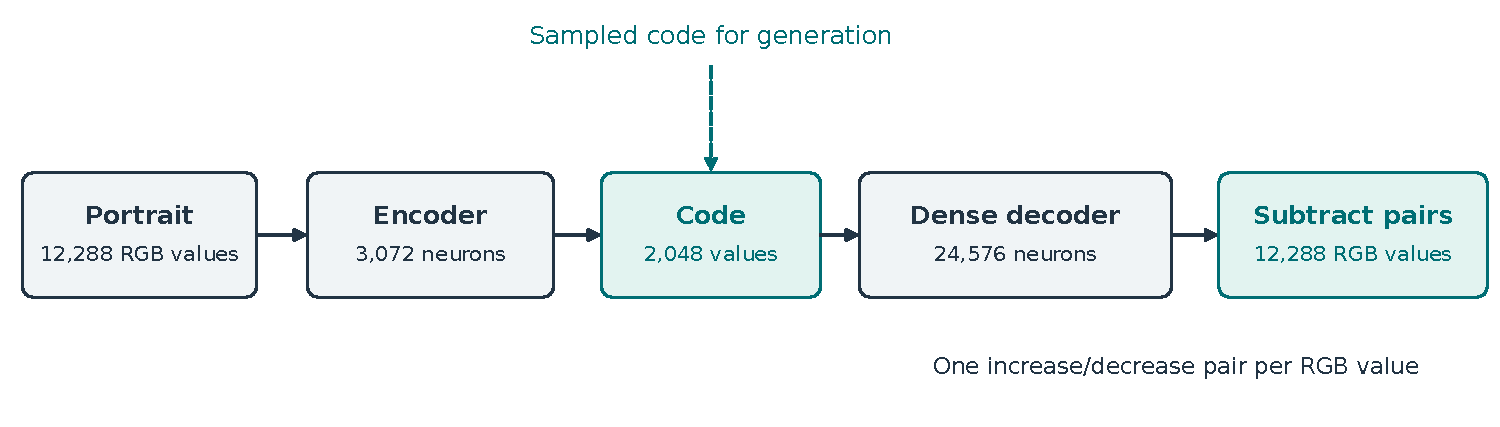
\includegraphics[width=\linewidth]{figures/autoencoder.pdf}
\caption{Class assignments in the CelebA autoencoder. At top, $h_1$ and $h_2$ are the signed activities of the first two neurons in each layer. Solid arrows show the dense forward connections. Dashed arrows show the error signs used in training. For example, output neurons 5,996 and 7,655 contribute $+e_{5996}$ and $-e_{7655}$ to the first bottleneck neuron. Its other 94 assigned classes supply the remaining terms. Below, the full network reconstructs the first test image.}
\label{fig:auto}
\end{figure}

The encoder maps the 12,288 input values through layers of 3,072 and 1,536 neurons to the 256-value embedding. The decoder has one hidden layer of 2,040 neurons and an output layer of 12,288 neurons. Each layer is fully connected to its immediate predecessor. In the output layer each neuron predicts its channel from its own activity magnitude (Eq.~\ref{eq:intensity}). The five dense layers contain 68,469,496 learned weights and biases.

In each of three pools of 1,024 neurons, the first encoder layer retains the signed activities of the 768 neurons with the largest magnitudes. The second encoder layer uses three Gaussian pools of 512 neurons with width 0.85. The bottleneck passes all 256 signed activities to the decoder. The decoder hidden layer uses three Gaussian pools of 680 neurons with width 0.50. Each hidden neuron receives 8, 16, 96 or 12 channel error signs in these four layers, respectively. The decoder hidden layer covers 12,240 channels, with each sign used twice. Every output neuron receives its own channel's sign directly.

All five layers use semi-implicit Hebbian Lion (Eqs.~\ref{eq:history} and~\ref{eq:update}) for three passes through the training set in minibatches of 128 images. The output layer starts at step $0.0008$ and the four hidden layers at $0.00008$. The schedule holds these steps for the first fifth of training, then decays them along a half cosine. We evaluate the initial weights and each half-pass checkpoint on 512 official validation images. The checkpoint at 2.5 passes has the lowest validation error.

\paragraph{Reconstruction.}
On the 19,962 official test images, the mean sum of squared RGB differences per image is 171.74. Each sum covers 12,288 intensities on the $[0,1]$ scale.

\paragraph{Generating with the decoder.}
\citet[Section~4]{ghosh2020} trained deterministic autoencoders by backpropagation, fitted a Gaussian mixture to the training embeddings, and decoded samples from that mixture to generate images, including CelebA images. \citet{samuth2024} sampled a low-rank Gaussian mixture fitted to the embeddings of a pretrained VQ-GAN autoencoder and refined each sample by nearest-neighbor matching before decoding.

For our Hebbian autoencoder, we fit a low-rank Gaussian mixture to the training embeddings after the network weights are fixed. We group the embeddings by $k$-means in the eight leading principal directions, after scaling each direction to unit variance. In each of the 16 groups we compute the mean $\mu_g$ and the leading 64 eigenvectors and eigenvalues of the covariance in the original 256-dimensional embedding space. To draw an image, choose group $g$ with probability proportional to its membership. Let $U_g$ contain its retained eigenvectors and $\Lambda_g$ its retained eigenvalues. Draw 64 independent standard normal values $\epsilon$ and decode
\begin{equation}
 z=\mu_g+0.85\,U_g\Lambda_g^{1/2}\epsilon .
\end{equation}
For the CelebA images shown here, we scale the standard deviations within each group by $0.85$. We pass each sampled embedding directly to the decoder.

\begin{figure}[ht]
\centering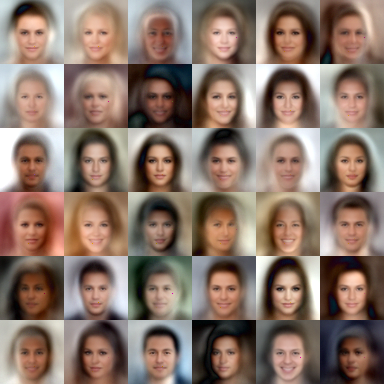
\includegraphics[width=.58\linewidth]{figures/celeba-generated.png}
\caption{CelebA decoder output for 36 consecutive draws from the fitted embedding distribution.}
\label{fig:faces}
\end{figure}

\section{Relation to other local learning methods}
The classifier of \citet{loverich2026} trains its layers jointly. A class decision based on the activities across layers supplies the teaching signals. In our regression networks, the sign of the final discrepancy supplies the teaching signal for each output. Groups of these signs teach hidden layers narrower than the output.

\citet{padmani2025} use Forward-Forward learning for regression. They train each layer by gradient descent to distinguish candidate pairs $(x,y)$ inside and outside a tolerance band around the target function. At inference they test multiple values of $y$ for one $x$ and average the accepted values. \citet{liu2026ffr} use competing neuron groups for ordered intervals of the target and combine estimates from several depths. Each hidden layer optimizes its own loss. A learned linear map of the group scores supplies the final layer's estimate and is trained by squared error with gradients confined to that map. In our coordinate regressor, the prediction at $x$ is the average of the layer estimates (Eq.~\ref{eq:output}). The final error sign for each output teaches the neurons contributing to that output at every depth.

\citet{qiao1992} used a global scalar error to train the hidden layer of a two-layer optical network without propagating derivatives through the output weights. Their hidden-layer rule suppresses an activity pattern after an error. Their output weights follow a gradient update derived from the output loss.

In the CIFAR-10 denoising autoencoder of \citet[Sections 4.3 and 5.2]{melchior2024}, Hebbian descent changes the loss used to train the output layer. It cancels the derivative of the output activation in the error signal. The network learns its output weights by gradient descent and uses backpropagation to train the earlier layers.

For autoencoders, \citet{hinton1988recirculation} trained the encoding and reconstruction connections together without backpropagation. They sent a mixture of the input and its reconstruction through the encoder a second time. The change in hidden activity taught the encoding connections. The reconstruction connections used the numerical change at the visible units, which gives a squared-error gradient for linear visible units.

\citet{teh2000} reconstruct face pairs without backpropagation. In their restricted Boltzmann machine, the same weights connect pixels to hidden units in both directions. Training compares their correlations on observed face pairs and on one-step reconstructions (their Fig.~1 and Eq.~3). \citet{ororbia2022} train a predictive coding model without backpropagation. The network repeatedly adjusts its hidden activities while an image is held at the input. Each layer predicts the one below it. The connections that produce the image learn from the activity above and the prediction error at the pixels. They used stochastic gradient descent for the local weight updates. After training they fitted a Gaussian mixture to the highest layer and sampled from it to generate images.

Our autoencoder trains the encoder and decoder together. The signs of the reconstruction errors from one forward pass teach the hidden neurons and the individual output neurons.

\section{Conclusion}
Supervised Hebbian class networks can train deep, fully connected networks for regression without backpropagation or gradient descent. A neuron can reinforce or suppress its activity using an error sign from the final prediction. All layers learn together, with each connection using the activities of the neurons it connects.

The same principle can be applied to scalar curve fitting, implicit representation and image generation. In the CelebA autoencoder, the signs of the reconstruction errors train the encoder and decoder together. After training, the decoder generates images from samples drawn from a distribution fitted to the learned embeddings.

To automate step selection across layers, we modified Hebbian Lion to adjust each neuron's step according to the sign agreement between its current and past Hebbian coactivities (Eq.~\ref{eq:agreement}). We used this rule for both the curve fit and the implicit image representation. The choice of update rule for supervised Hebbian class networks warrants further study.

\bibliographystyle{tmlr}
\bibliography{references}
\end{document}
